\section{Case-Studies}
In this section we present two case-studies in simulating the \textit{Prisoners Dilemma} and \textit{Heroes \& Cowards} games for discussing the effect of using different update-strategies. As already emphasised both are of different nature. The first one is a discrete game, played at discrete time-steps. The second one is a continuous game where each agent is continuously playing. This has profound implications on the simulation results as will is shown below. The results show that depending on the type of model the results can be very different when using different update-strategies as happening in the case of \textit{Prisoners Dilemma}. Results of other models seem to be stable under varying update-strategies as is the case with \textit{Heroes \& Cowards}.

\begin{table*}
	\begin{tabular}{c c c}
		& Prisoners Dilemma & Heroes \& Cowards \\ 

		\textit{\rotatebox{90}{sequential strategy}}
		&
		\begin{subfigure}[b]{0.4\textwidth}
			\centering
			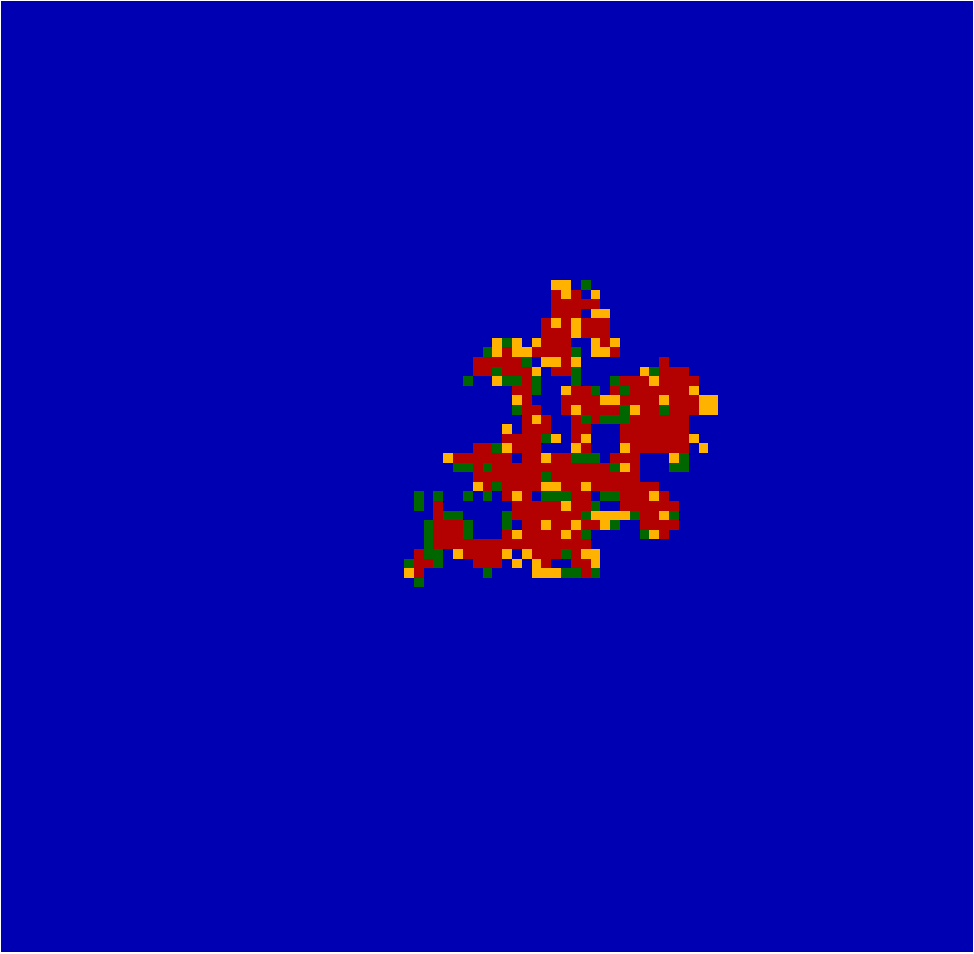
\includegraphics[width=.7\textwidth, angle=0]{./fig/seq_99x99_217steps_MSG_java.png}
			\caption{}
			\label{fig:pd_seq}
		\end{subfigure}
    	&
		\begin{subfigure}[b]{0.4\textwidth}
			\centering
			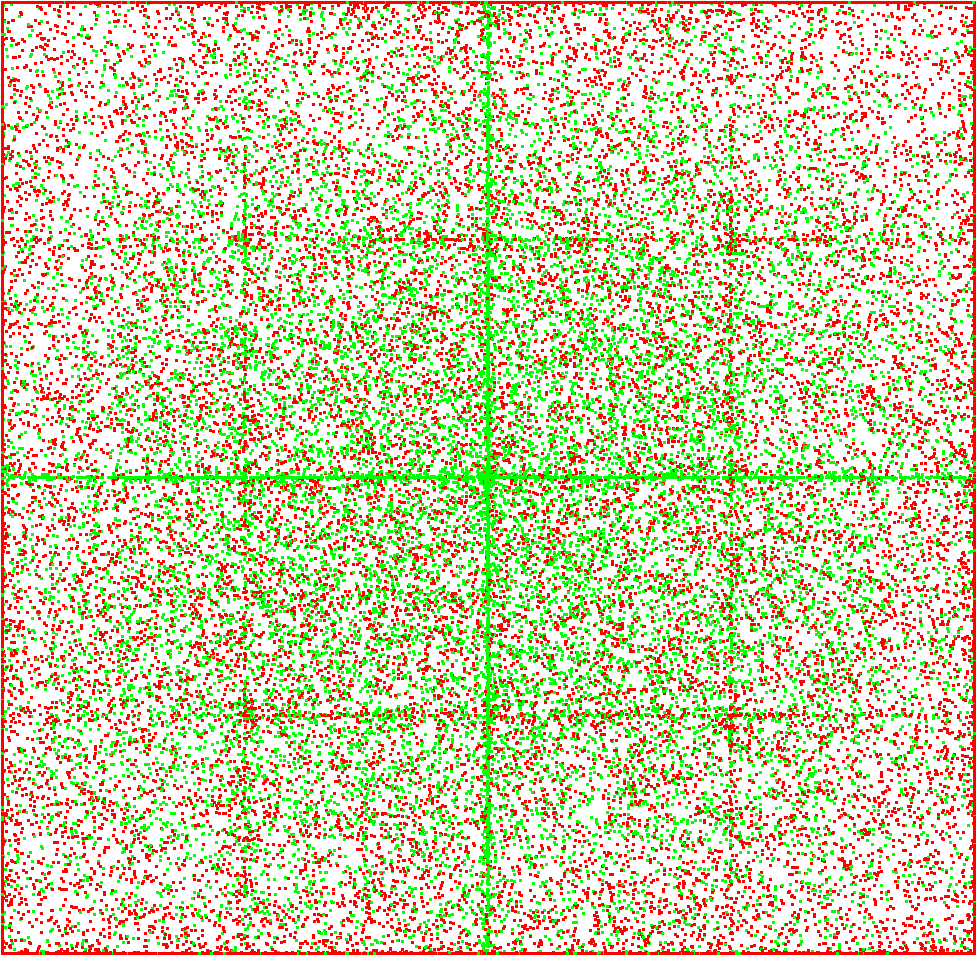
\includegraphics[width=.7\textwidth, angle=0]{./fig/seq_HAC_100_000_500steps_java.png}
			\caption{}
			\label{fig:hac_seq}
		\end{subfigure}
    	\\
    	
    	\textit{\rotatebox{90}{parallel strategy}}
		&
		\begin{subfigure}[b]{0.4\textwidth}
			\centering
			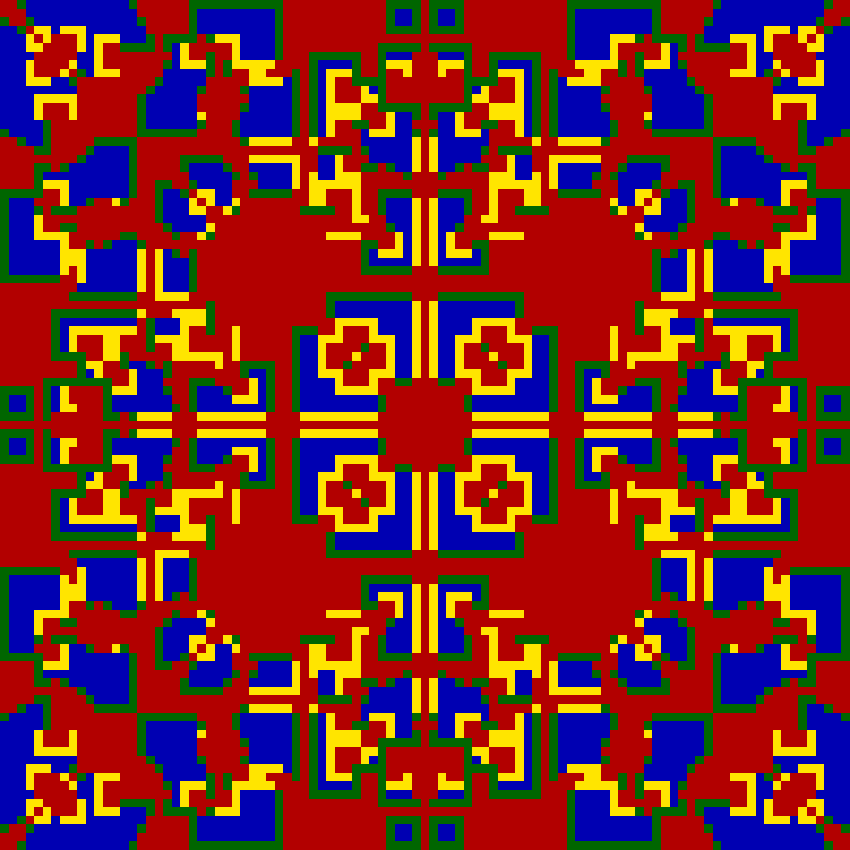
\includegraphics[width=.7\textwidth, angle=0]{./fig/par_99x99_436steps_MSG_haskell.png}
			\caption{}
			\label{fig:pd_par}
		\end{subfigure}
    	&
		\begin{subfigure}[b]{0.4\textwidth}
			\centering
			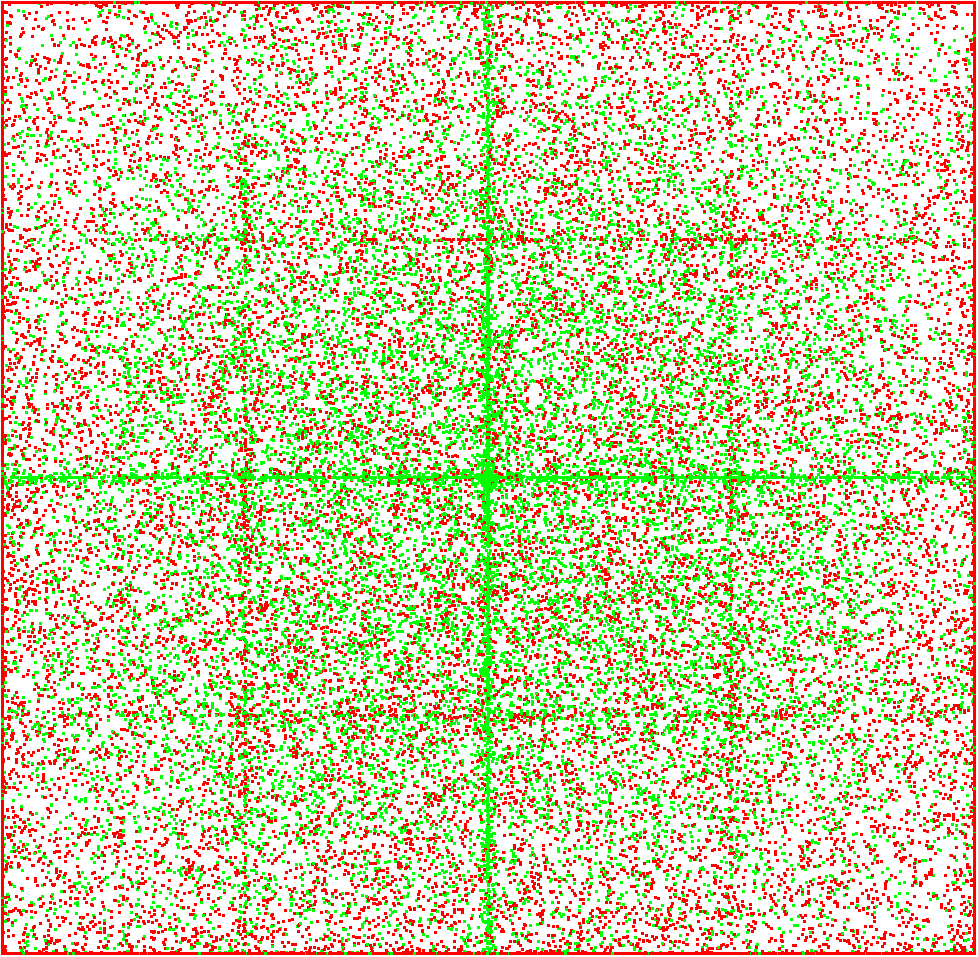
\includegraphics[width=.7\textwidth, angle=0]{./fig/par_HAC_100_000_500steps_java.png}
			\caption{}
			\label{fig:hac_par}
		\end{subfigure}
    	\\
    	
    	\textit{\rotatebox{90}{concurrent strategy}}
		&
		\begin{subfigure}[b]{0.4\textwidth}
			\centering
			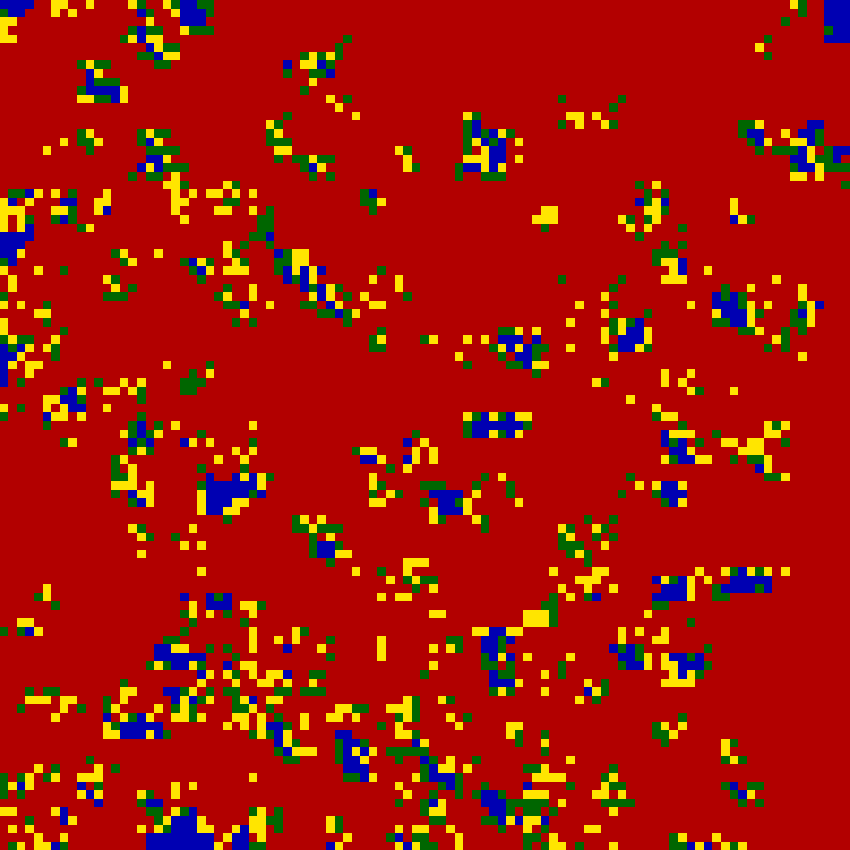
\includegraphics[width=.7\textwidth, angle=0]{./fig/con_99x99_436steps_MSG_haskell.png}
			\caption{}
			\label{fig:pd_con}
		\end{subfigure}
    	&
		\begin{subfigure}[b]{0.4\textwidth}
			\centering
			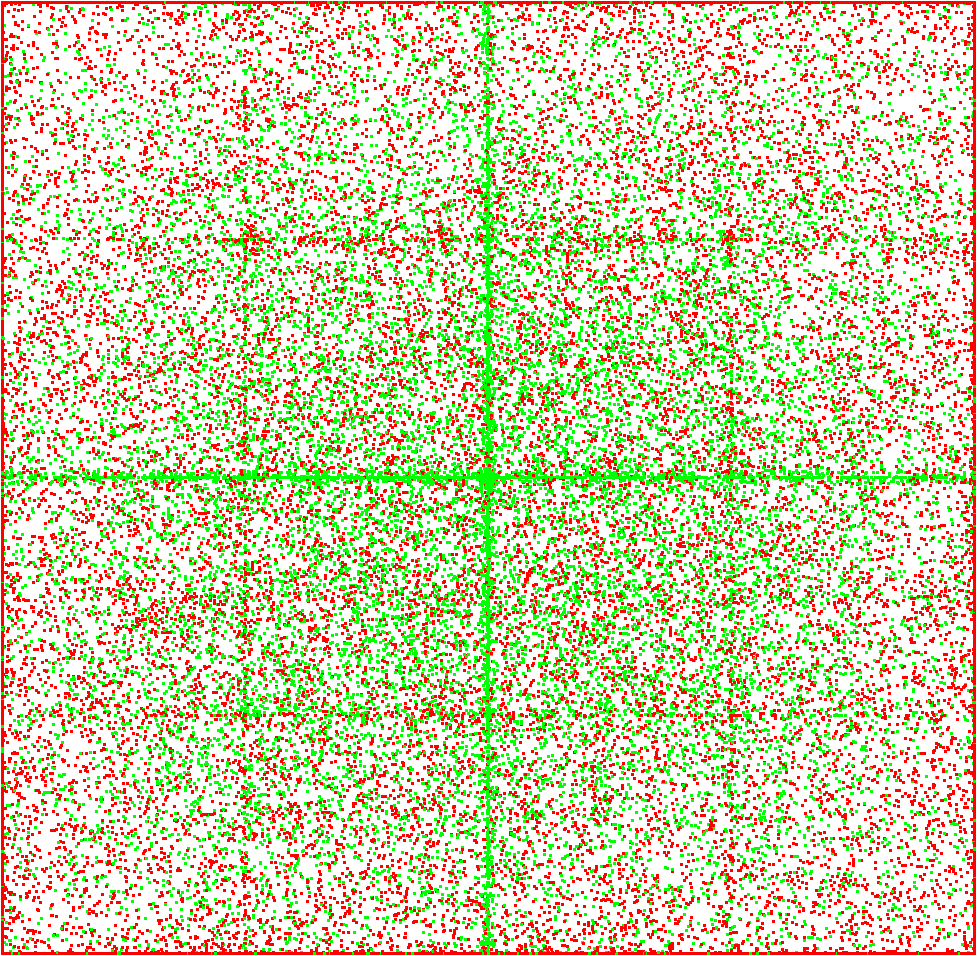
\includegraphics[width=.7\textwidth, angle=0]{./fig/con_HAC_100_000_500steps_java.png}
			\caption{}
			\label{fig:hac_con}
		\end{subfigure}
    	\\ 
    	
    	\textit{\rotatebox{90}{actor strategy}}
		&
		\begin{subfigure}[b]{0.4\textwidth}
			\centering
			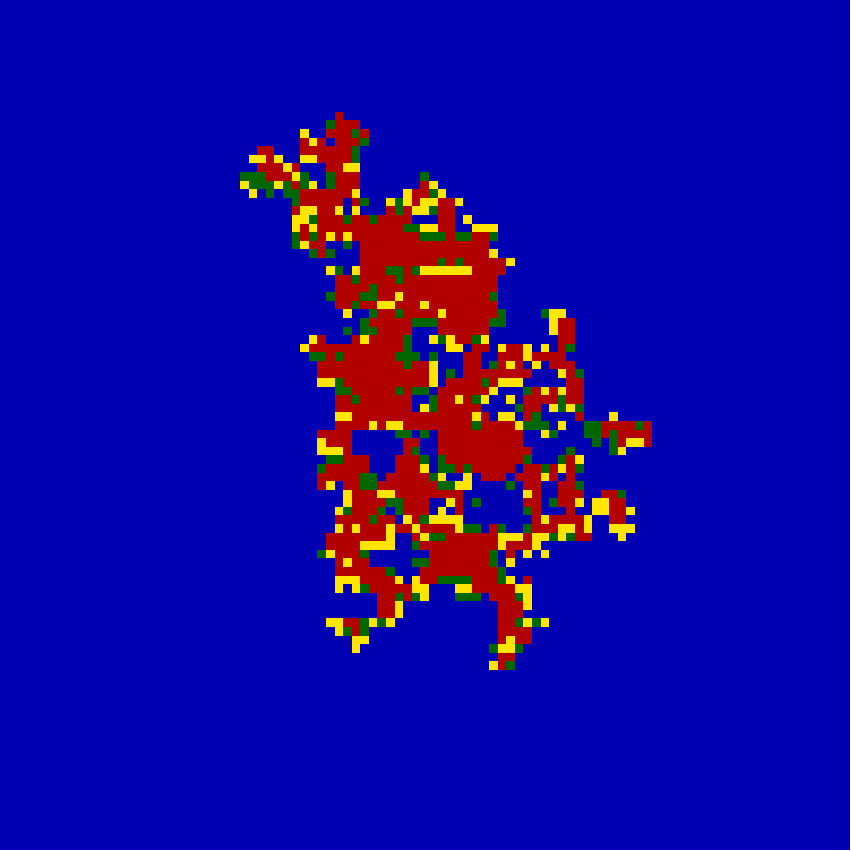
\includegraphics[width=.7\textwidth, angle=0]{./fig/act_99x99_436steps_MSG_haskell.png}
			\caption{}
			\label{fig:pd_act}
		\end{subfigure}
    	& 
		\begin{subfigure}[b]{0.4\textwidth}
			\centering
			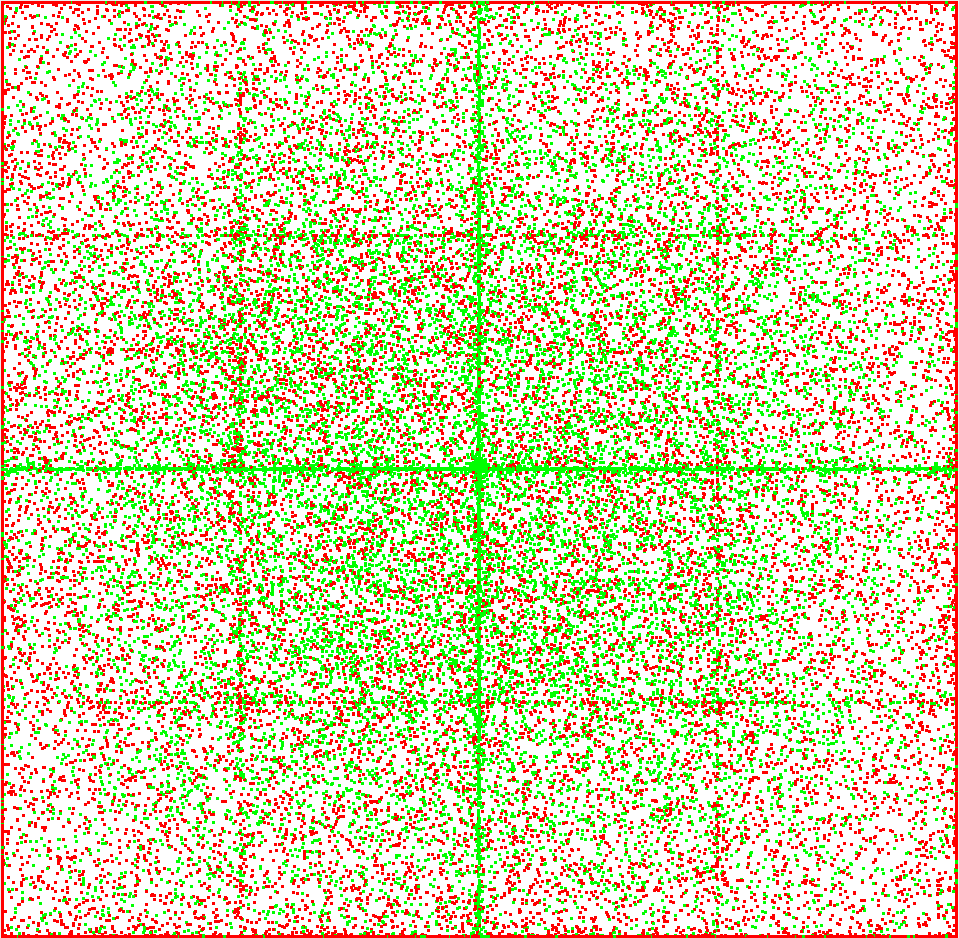
\includegraphics[width=.7\textwidth, angle=0]{./fig/act_HAC_100_000_500steps_scala.png}
			\caption{}
			\label{fig:hac_act}
		\end{subfigure}

	\end{tabular}
	
	\caption{\small Effect on results simulating the Prisoners Dilemma and Heroes \& Cowards with all four update-strategies.} 
	\label{fig:results}
\end{table*}

%\begin{figure*}
%
%	 \centering
	
%    \begin{subfigure}[b]{0.4\textwidth}
%			\centering
%       	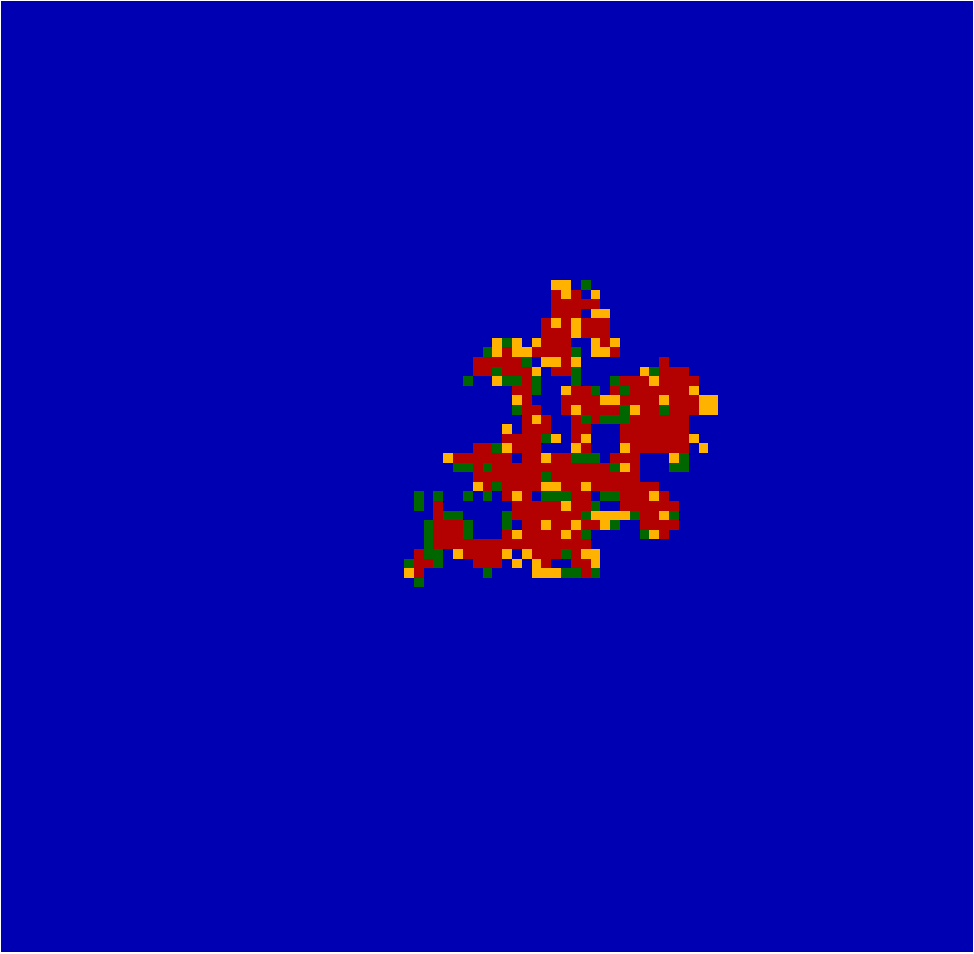
\includegraphics[width=.7\textwidth, angle=0]{./fig/seq_99x99_217steps_MSG_java.png}
%        \caption{\textit{sequential} Prisoners Dilemma}
%        \label{fig:pd_seq}
%    \end{subfigure}
%    \begin{subfigure}[b]{0.4\textwidth}
%		\centering
%        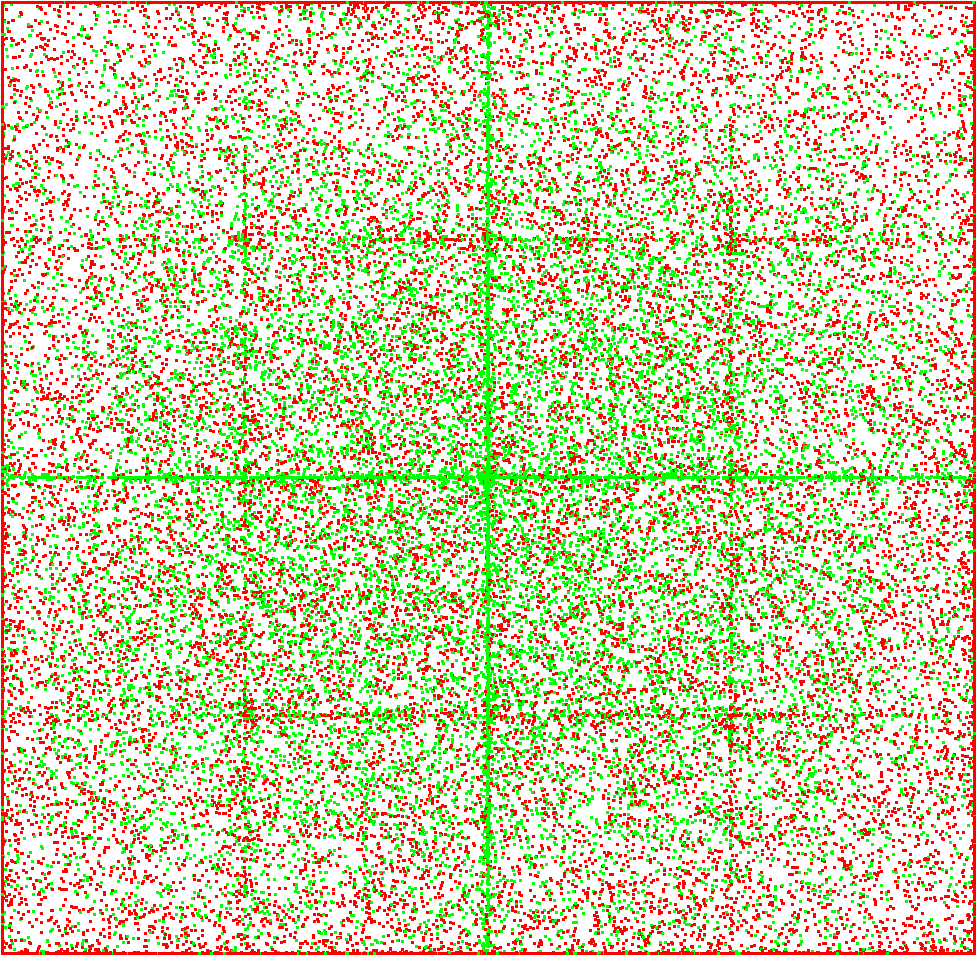
\includegraphics[width=.7\textwidth, angle=0]{./fig/seq_HAC_100_000_500steps_java.png}
%        \caption{\textit{sequential} Heroes \& Cowards}
%        \label{fig:hac_seq}
%    \end{subfigure}
%       

%    \begin{subfigure}[b]{0.4\textwidth}
%		\centering
%       	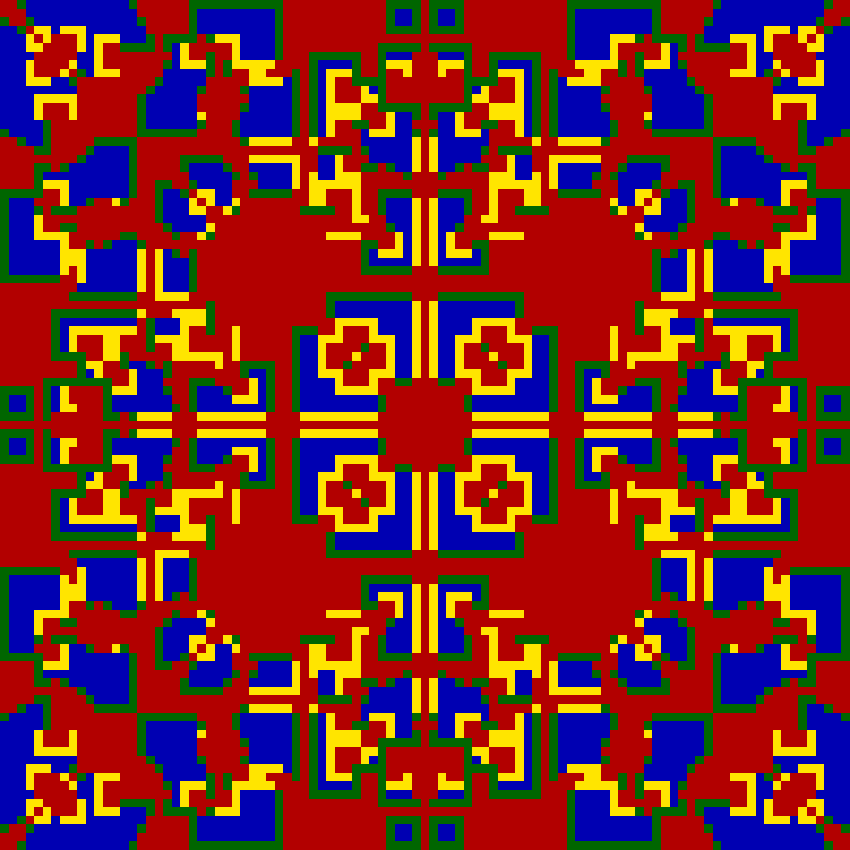
\includegraphics[width=.7\textwidth, angle=0]{./fig/par_99x99_436steps_MSG_haskell.png}
%        \caption{\textit{parallel} Prisoners Dilemma}
%        \label{fig:pd_par}
%    \end{subfigure}
%    \begin{subfigure}[b]{0.4\textwidth}
%    	\centering
%        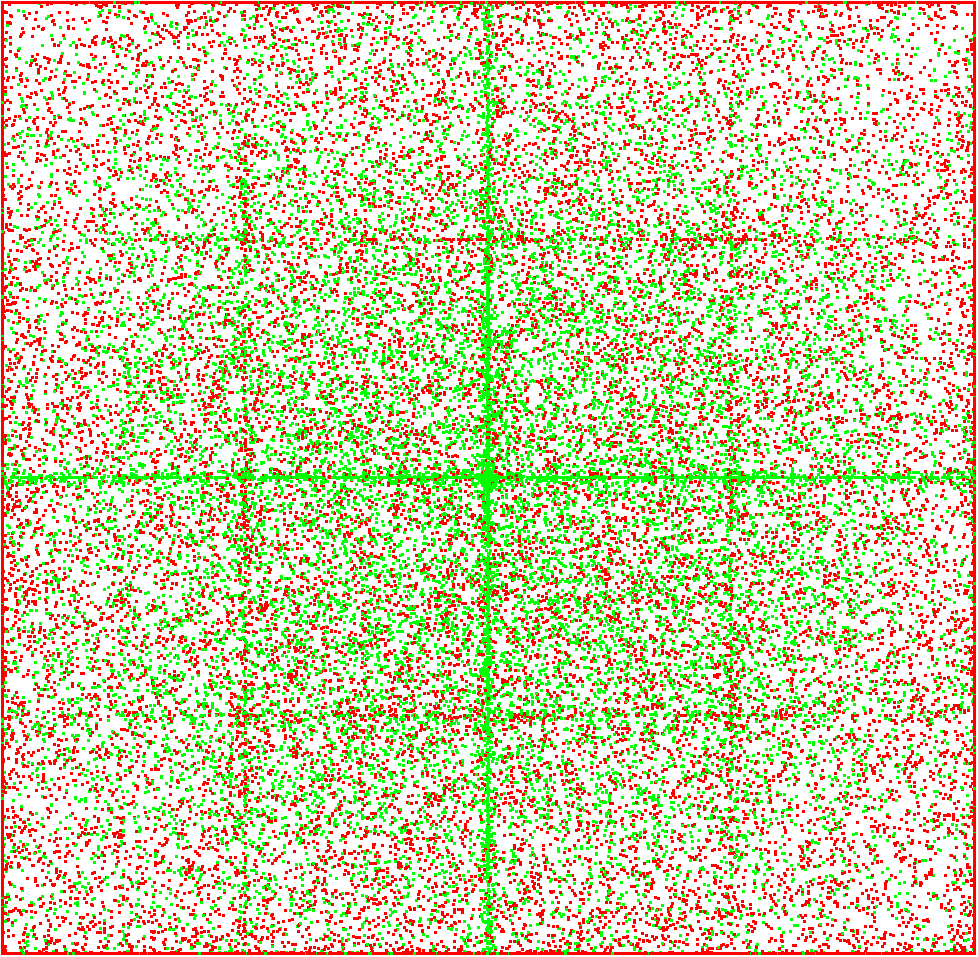
\includegraphics[width=.7\textwidth, angle=0]{./fig/par_HAC_100_000_500steps_java.png}
%        \caption{\textit{parallel} Heroes \& Cowards}
%        \label{fig:hac_par}
%    \end{subfigure}
%        
%
%    \begin{subfigure}[b]{0.4\textwidth}
%		\centering
%       	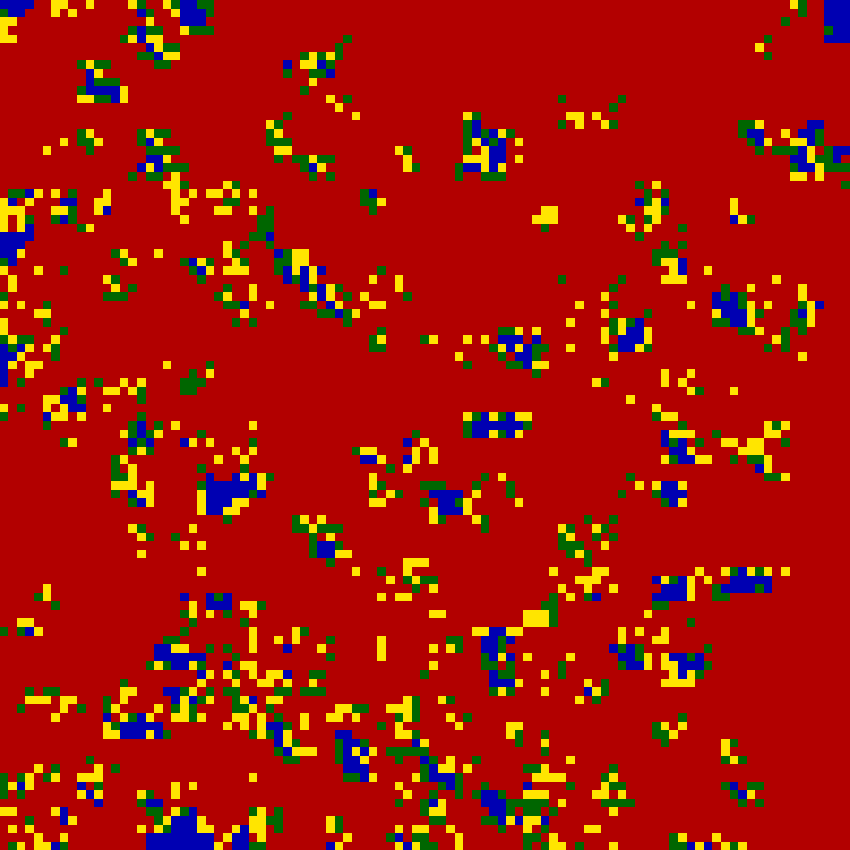
\includegraphics[width=.7\textwidth, angle=0]{./fig/con_99x99_436steps_MSG_haskell.png}
%        \caption{\textit{concurrent} Prisoners Dilemma}
%        \label{fig:pd_con}
%    \end{subfigure}
%    \begin{subfigure}[b]{0.4\textwidth}
%    	\centering
%        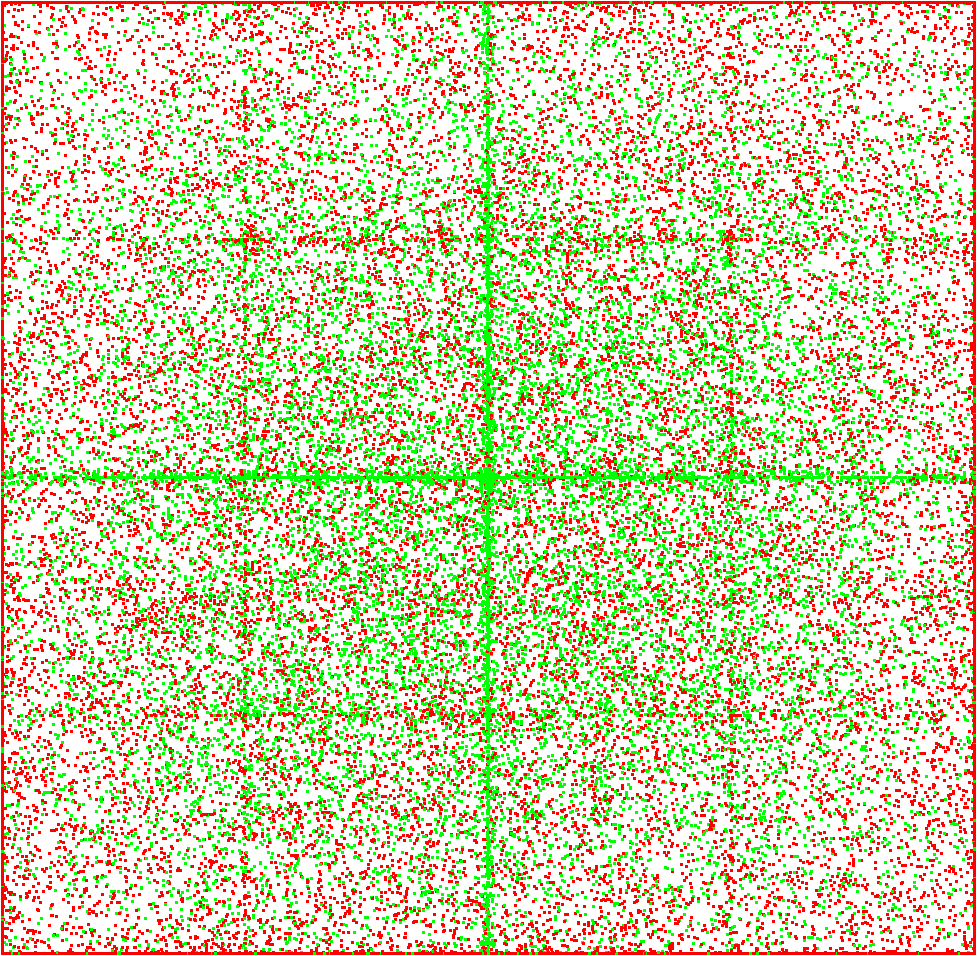
\includegraphics[width=.7\textwidth, angle=0]{./fig/con_HAC_100_000_500steps_java.png}
%        \caption{\textit{concurrent} Heroes \& Cowards}
%        \label{fig:hac_con}
%    \end{subfigure}
%
%
%    \begin{subfigure}[b]{0.4\textwidth}
%		\centering
%       	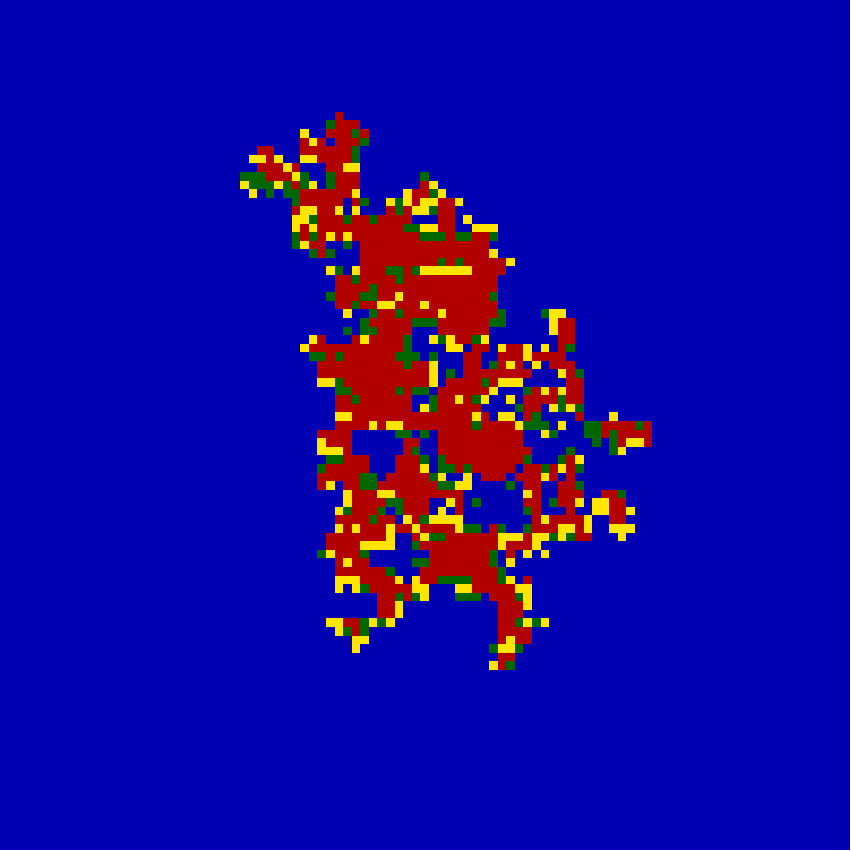
\includegraphics[width=.7\textwidth, angle=0]{./fig/act_99x99_436steps_MSG_haskell.png}
%        \caption{\textit{actor} Prisoners Dilemma}
%        \label{fig:pd_act}
%    \end{subfigure}  
%    \begin{subfigure}[b]{0.4\textwidth}
%    	\centering
%        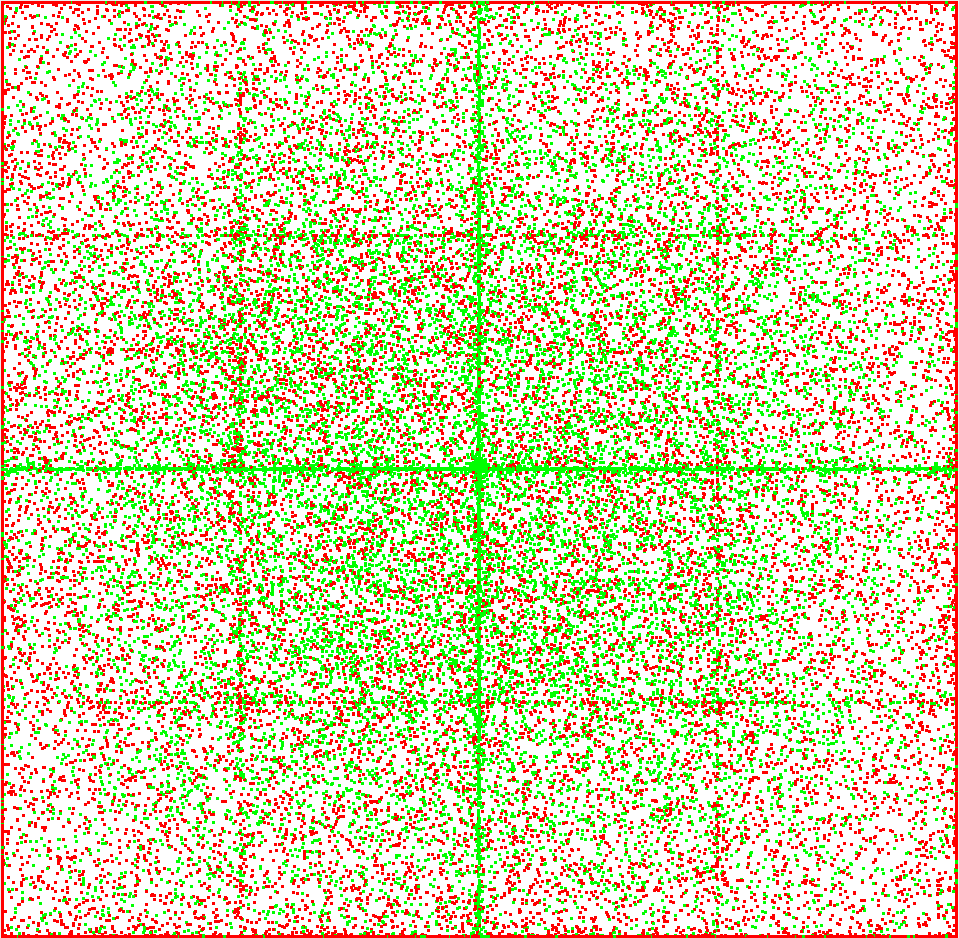
\includegraphics[width=.7\textwidth, angle=0]{./fig/act_HAC_100_000_500steps_scala.png}
%        \caption{\textit{actor} Heroes \& Cowards}
%        \label{fig:hac_act}
%    \end{subfigure}

%	\caption{\small Results of Prisoners Dilemma and Heroes \& Cowards with all four update-strategies.} 
%	\label{fig:results}
%\end{figure*}

\subsection{Prisoners Dilemma}
The results as seen in the left column of figure \ref{fig:results} were created using the Haskell implementation with the same configuration as reported in the original paper: a 99x99 grid with all cooperators except one defector at the center, running for 217 steps. When comparing the pictures with the one from the original paper seen in figure \ref{fig:sync_patterns} the only update-strategy which is able to reproduce the matching result is the \textit{parallel strategy} - all the others clearly fail to reproduce the pattern. From this we can deduce that only the \textit{parallel strategy} is suitable to simulate this model because only that strategy is the one which renders the results of the original paper, meaning it is the 'correct' strategy for this model. The reason why the other strategies fail to reproduce the pattern is due to the non-parallel and unsynchronized way that information spreads through the grid. In the \textit{sequential strategy} the agents further ahead in the queue play the game earlier and influence the neighbourhood so agents which play the game later find already messages from earlier agents in their queue thus acting differently based upon these informations. In the \textit{concurrent} and \textit{actor strategy} the agents run in parallel but changes are visible immediately and concurrently, leading to the same non-structural patterns as in the \textit{sequential} one. This is not the case in the \textit{parallel strategy}  where, in every step, all agents play the game at the same time based on the frozen state of the previous step, leading to a synchronized update as required by the model. Note that the \textit{concurrent} and \textit{actor strategy} produce different results on every run due to the inherent non-deterministic event-ordering introduce by concurrency. As there are no global time-steps in the \textit{actor strategy}, to calculate 45 steps we just waited until the first agent arrived at a local time of 217 and then rendered the result.

TODO: when having queued messages instead of immediate messaging in SEQ (exact same implementation as in parallel) then we get the same result as in parallel version.

TODO: how did implementation happen? at each step send state to neighbours, if an agent received all states it can calculate the local payoff and send it to all neighbours, if an agent received all local payoffs it can decide which is the best and can change its state. In parallel one can not answer in the same step but answer will show up in the next step => need twice as many steps.

\subsection{Heroes \& Cowards}
The results as seen in the right column of figure \ref{fig:results} were created using the Java and Scala implementations with 100.000 agents where 25\% of them were heroes after 500 steps. Although the individual agent-positions of runs with the same configuration differ between update-strategies the cross-patterns are forming in all four update-strategies. For the patterns to emerge it is important to have significant more cowards than heroes and to have more than 75.000 agents - we went for 100.000 because then the patterns are really prominent. We can conclude that the \textit{Heroes \& Cowards} model seems to be robust to the selection of its update-strategy and that its emergent property - the formation of the cross - is stable under differing strategies. To test the \textit{actor strategy} with this high number of agents we used our implementation in Scala with the Actor-library as Java is not able to have this high number of threads and our Haskell implementation suffers from performance issues.


TODO: how did implementation happen? every agent asks its friend and enemy in every step for their position